Во второй главе рассматриваются архитектурные решения, за счет которых
генератор масштабируется по числу партиций и рабочих потоков, но при этом
сохраняет детерминированность результата. Основное внимание уделяется общей
схеме работы программы, независимому запуску генераторов для произвольной
партиции, архитектуре слоя сериализации, в которой параллельное построение
батчей сочетается с линейным порядком записи, и разделению генераторного ядра
и слоя сериализации.

\subsection{Архитектурные требования к масштабируемой генерации}

Базовое требование к архитектуре генератора состоит в сохранении совместимости
со спецификацией TPC-H~\cite{tpch-spec}. Это означает, что при
одинаковых параметрах запуска должны воспроизводиться те же ключевые
зависимости, распределения значений и итоговый логический порядок строк
независимо от числа потоков и разбиения таблицы на партиции.

Второе требование связано с масштабируемостью. Параллельная генерация не должна
опираться на последовательный прогон всех предшествующих строк, поскольку в
таком случае стоимость подготовки очередной партиции росла бы пропорционально
ее смещению относительно начала таблицы. Следовательно, архитектура должна
поддерживать быстрый переход к произвольной строке без симуляции всего
префикса.

Третье требование относится к записи результата. Слой сериализации должен
оставаться отделенным от ядра генерации и принимать готовые батчи
Apache Arrow~\cite{apache-arrow}. При этом для режимов записи в один
файл требуется обеспечить одновременно три свойства: параллельную генерацию
партиций, линейный порядок данных в итоговом артефакте и детерминированность
результата.

\subsection{Общая идея алгоритма}

Функционирование программы организовано как последовательность этапов выбора
сценария генерации, формирования таблиц и записи результата.

На первом этапе программа обрабатывает параметры командной строки, определяющие
масштаб генерации, состав таблиц, формат вывода и путь размещения результата.
После этого выполняется регистрация метаданных таблиц и выбирается требуемый
драйвер сериализации.

На втором этапе для каждой выбранной таблицы определяется объем данных и схема
разбиения на логические партиции. Далее для каждой партиции запускается
генератор, формирующий значения атрибутов по детерминированным правилам
TPC-H.

На третьем этапе сгенерированные значения накапливаются и объединяются в батчи
для увеличения пропускной способности. После этого батчи передаются слою
сериализации, который сохраняет результат в требуемом формате хранения.

\subsection{Параллельная генерация на основе перемотки линейного генератора}

\subsubsection{Математическая модель генератора}

В основе большинства генераторов значений TPC-H лежит линейный
конгруэнтный генератор без аддитивного слагаемого. Для каждой последовательности
используется рекуррентное соотношение
\begin{equation}
    X_{n+1} = a X_n \bmod m,
\end{equation}
где для 32-разрядного варианта TPC-H принимаются
\begin{equation}
    a = 16807, \qquad m = 2^{31} - 1.
\end{equation}

Отдельные генераторы атрибутов используют собственные начальные значения. Начальное состояние конкретного столбца
дополнительно смещается относительно базового значения, поэтому разные атрибуты
не разделяют одну и ту же последовательность случайных чисел. Если генератор
$g$ расходует $s_g$ значений на одну строку, то начало строки с номером $r$
соответствует состоянию
\begin{equation}
    X^{(g)}_{r s_g}.
\end{equation}

Из этого следует, что для партиции, начинающейся со строки $r_0$, генератору
не требуется воспроизводить весь префикс таблицы. Достаточно перейти к
состоянию
\begin{equation}
    X^{(g)}_{r_0 s_g},
\end{equation}
после чего строки диапазона $[r_0, r_1)$ могут строиться независимо от других
партиций. Если внутри текущей строки уже было использовано $u_g$ значений, то
для перехода к следующей строке выполняется добор
\begin{equation}
    \Delta_g = s_g - u_g,
\end{equation}
что восстанавливает фиксированный шаг по строкам и сохраняет совместимость с
эталонным порядком использования случайных чисел.

\subsubsection{Алгоритм быстрой перемотки и асимптотика}

Поскольку используемый генератор является мультипликативным, переход на $k$
шагов вперед выражается в замкнутой форме:
\begin{equation}
    X_{n+k} = a^k X_n \bmod m.
\end{equation}
Тем самым задача перемотки сводится к вычислению $a^k \bmod m$.

\begin{lstlisting}[style=reportpseudocodeinline,caption={Перемотка линейного генератора}]
func skip_ahead(state, steps, multiplier, modulus):
    factor = multiplier
    result = state
    remaining = steps

    while remaining > 0:
        if remaining mod 2 == 1:
            result = (result * factor) mod modulus

        factor = (factor * factor) mod modulus
        remaining = remaining // 2

    return result
\end{lstlisting}

Такой алгоритм выполняется за $O(\log k)$ при $O(1)$ дополнительной памяти,
тогда как последовательный пропуск потребовал бы $O(k)$ шагов. Поэтому рабочий
поток может сразу восстановить состояние генератора для начала своей партиции и
строить строки независимо от предшествующих партиций. Именно это делает
параллельную генерацию практически масштабируемой по числу партиций.

\subsection{Архитектура слоя сериализации}

\subsubsection{Форматно-зависимые компоненты записи}

Слой сериализации проектируется как набор форматно-зависимых
\textit{writer}-компонентов, принимающих на вход готовые батчи
Apache Arrow~\cite{apache-arrow}. Для одних колонoчных форматов
используются файловые компоненты записи, поддерживающие как запись набора
файлов-партиций, так и запись в один итоговый файл. Для других колонoчных
форматов используются отдельные упорядоченные компоненты записи, передающие
батчи во внешний рантайм формата.

Такое разделение позволяет сохранить единое ядро генерации и менять только
последний этап конвейера. Генераторы таблиц всегда формируют один и тот же тип
внутреннего результата, а различия между форматами и способами размещения
данных локализованы внутри специализированных компонентов записи.

\subsubsection{Линейный и детерминированный режим записи}

В режиме раздельной записи партиций каждая партиция записывается собственным
компонентом записи в отдельный файл. Такой режим хорошо масштабируется по числу
рабочих потоков, поскольку между потоками отсутствует конкуренция за общий
выходной артефакт.

Более сложной является архитектура режима упорядоченной записи в один итоговый
файл. Здесь несколько производителей параллельно генерируют батчи партиций и
передают их через ограниченную очередь Вьюкова MPSC
(\textit{multi-producer, single-consumer})~\cite{vyukov-mpsc}. На стороне потребителя поддерживаются буфер готовых
партиций и указатель ожидаемой партиции, задающий номер следующей
партиции, которую разрешено зафиксировать в итоговом файле.

Если сообщение приходит от ожидаемой партиции, ее батчи сразу передаются в
единый компонент записи. Если батч относится к более поздней партиции, он
временно буферизуется до тех пор, пока не будут полностью записаны все
предшествующие партиции. Тем самым итоговый файл всегда формируется в порядке
номеров партиций, а не в порядке фактической готовности рабочих потоков.

Схема ручного упорядочения партиций для форматов с упорядоченной записью в
один файл приведена на рисунке \ref{fig:serialization-flow}. На ней показано,
как параллельные производители передают сообщения в общую очередь, а
потребитель линейно фиксирует партиции в порядке их номеров.

\begin{figure}[ht]
\centering
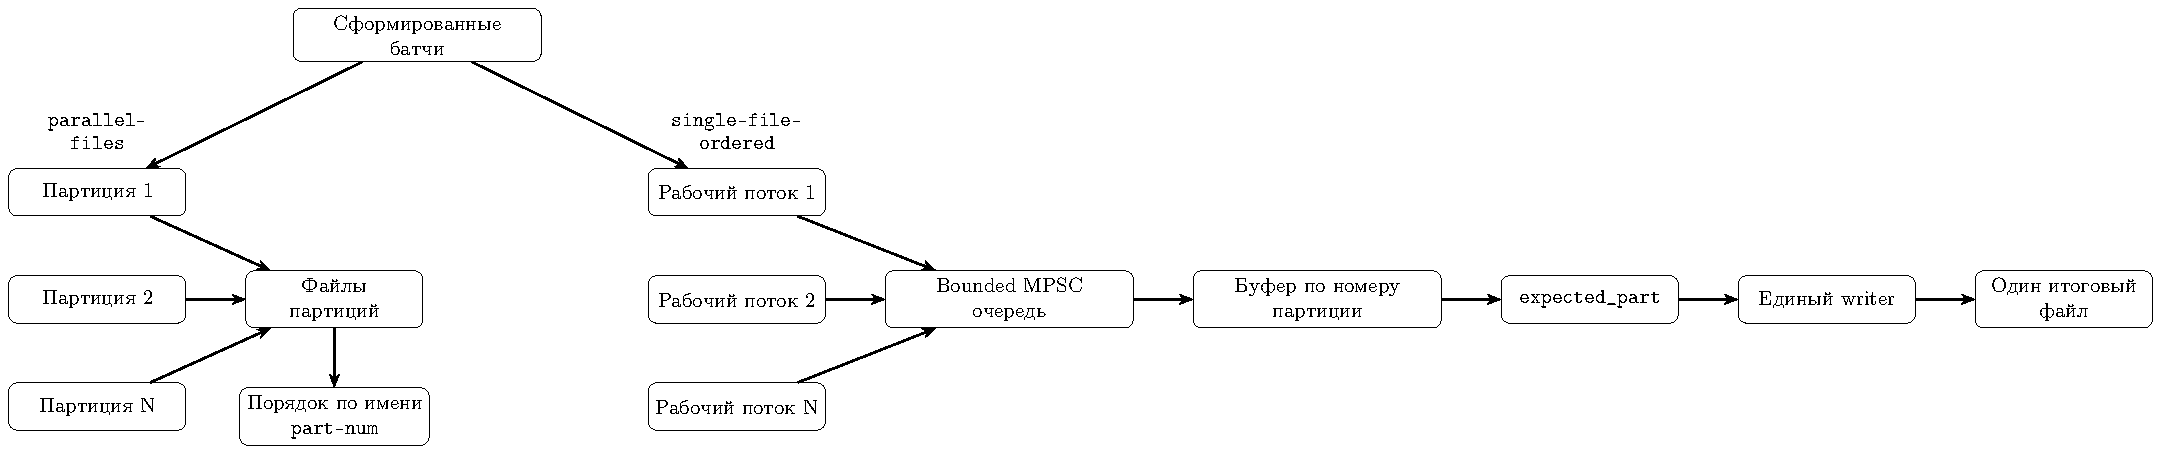
\includegraphics[width=\textwidth]{../expl-note/image/serialization-diagram.pdf}
\caption{Схема ручного упорядочения партиций для форматов с записью в один файл}
\label{fig:serialization-flow}
\end{figure}

Линейность обеспечивается самим инвариантом ожидаемой партиции: никакая
партиция не может быть записана раньше всех предшествующих. Детерминированность
следует из того, что содержимое каждой партиции уже фиксировано на этапе
генерации, а порядок записи определяется только номером партиции. Выбор
очереди Вьюкова MPSC здесь важен как практический способ совместить
высокий уровень параллелизма производителей с одним упорядочивающим
потребителем.

\subsection{Разделение модулей генерации и сериализации}

Дополнительное архитектурное решение состоит в явном разделении модуля
генерации и слоя сериализации. Генератор отвечает только за построение строк,
партиций и батчей Apache Arrow, тогда как сериализация начинается
только после формирования очередного батча. Благодаря этому граница между
компонентами проходит по устойчивому внутреннему представлению данных, а не по
формату выходного файла.

Такое разделение оказалось важным не только для поддержки нескольких форматов
хранения, но и для встраиваемого сценария. В расширении для
DuckDB~\cite{schengen-duckdb-repo,duckdb-extensions} используется
только генераторная часть конвейера: вместо передачи батчей в файловый
компонент записи они сразу экспортируются во внешний табличный источник. Тем
самым архитектурное отделение сериализации от генерации позволяет использовать
один и тот же генератор и как автономную утилиту записи файлов, и как
внутрипамятный источник данных для аналитической СУБД.

\subsection*{Выводы по главе}
\addcontentsline{toc}{subsection}{Выводы по главе}

Во второй главе выделены два архитектурных решения, определяющих
масштабируемость генератора. Первое из них состоит в быстрой перемотке
линейного генератора случайных чисел, благодаря которой партиции могут
обрабатываться независимо друг от друга. Второе связано с построением слоя
сериализации как набора форматно-зависимых компонентов записи и
использованием очереди MPSC для упорядоченной записи в один файл.

Тем самым на архитектурном уровне обеспечиваются параллельное масштабирование
по числу партиций, линейный детерминированный порядок результата при записи и
возможность повторного использования только генераторной части конвейера во
встраиваемом сценарии.
